\chapter{Methode}
\label{ch:Methode}
Im Kapitel \fullref{ch:Methode} werden die verwendeten Methoden vorgestellt. Dabei geht es um die Definition der
Problemstellung, sowie der Projektabgrenzung.

\section{Vorgehensmodell}
\label{sec:Vorgehensmodell}
Dieses Projekt wurde mittels einem explorativen Vorgehensmodell umgesetzt, da sich dieses Modell optimal für ein
Innovation- / Forschungsprojekt anwenden lässt. Ausserdem wird in diesem Modell die kreative Problemlösung mittels
mehreren Lernzyklen gefördert, was in einem Innovationsprojekt ein Muss ist. Dieses Modell wird in Grafik
\ref{fig:Meilensteinplanung} dargestellt.
\newline
\newline
In einer ersten Phase, der Initialisierungsphase, wird das Projekt genauer untersucht sowie allfällige Fragen und
Unwissenheiten geklärt. Nach der Initialisierungsphase sollte klar sein, was genau mit der Arbeit erreicht werden soll
und welches die grössten Schwierigkeiten sind. 
\newline
\newline
Anschliessend gibt es eine divergierende Ideenfindungsphase, in der der aktuelle Stand der Technik untersucht wird und
verschiedene Ansätze erforscht werden. In dieser Phase sollten auch verschiedene Experimente durchgeführt werden, um die
Machbarkeit besser zu beurteilen. Nach dieser Phase sollte klar sein, welche Ansätze in Frage kommen, um das Projekt
umzusetzen.
\newline
\newline
Nach der divergierenden Phase kommt die konvergierende Ideenfindungsphase, in der das Ziel ist, aus den vorher
erforschten Methoden wenige auszuwählen und genauer zu untersuchen. So kann die Anwendbarkeit auf das Projekt beurteilt
werden. Nach dieser Phase sollten nur noch etwa 1-2 Ideen bestehen, welche die Problemstellung optimal angehen und einen
vielversprechenden Ansatz zur Lösung dieser bieten.
\newline
\newline
Die letzte Phase in diesem Vorgehensmodell ist die Umsetzungsphase, diese beinhaltet die komplette Umsetzung der Idee
mittels den erforschten Ideen aus den vorherigen Phasen. Dabei geht es vor allem darum die Problemstellung so weit wie
möglich zu lösen und auch Vorschläge für die Umsetzung anderer Ideen in der gleichen Domäne zu geben. Nach der
Umsetzungsphase sollte das Projekt abgeschlossen sein und ein Prototyp sowie eine klare Forschung zum jeweiligen
Themengebiet ersichtlich sein.
\begin{figure}[H]
	\centering
	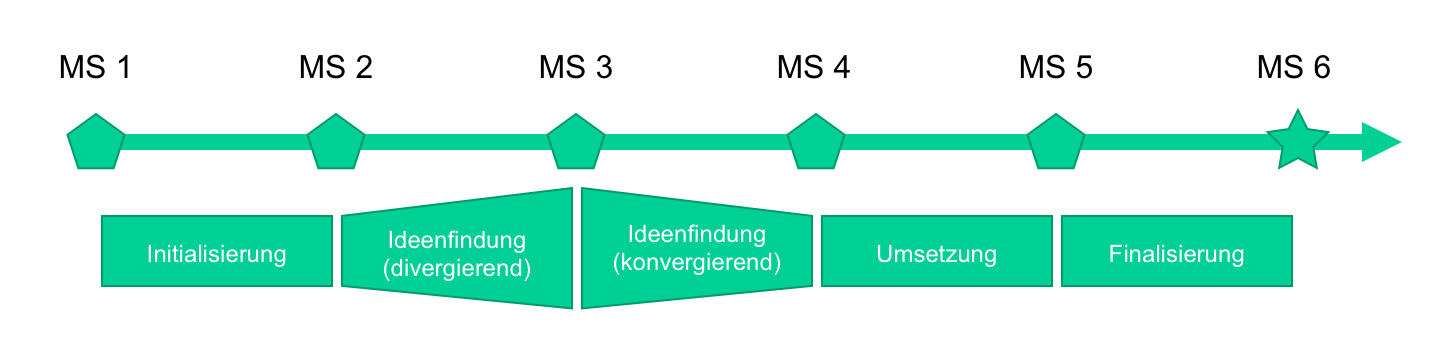
\includegraphics[scale=0.3]{Meilensteinplanung}
	\caption{Meilensteinplanung}
	\label{fig:Meilensteinplanung}
\end{figure}
\noindent

\subsection{Meilensteinplanung}
\label{sec:Meilensteinplanung}
Die Meilensteinplanung ist im explorativen Vorgehensmodell naheliegend, nach jeder abgeschlossenen Phase gibt es einen
neuen Meilenstein, sowie beim Start und bei der Abgabe. Demnach gibt es insgesamt $ 6 $ Meilensteine, die erreicht
werden sollen. Die Termine der Meilensteine ergeben sich aus der Zeitplanung des Herbstsemesters an der HSLU und den
Rahmenbedingungen des Moduls \flqq Wirtschaftsprojekt\frqq. Die detaillierten Berichte zu den einzelnen Meilensteinen
können im Anhang eingesehen werden unter \fullref{app:meilensteinberichte}.
\begin{itemize}
	\setlength\itemsep{0em}
	\item \textbf{M1: 26. September 2019}, Start des Projektes
	\item \textbf{M2: 10. Oktober 2019}, Ende Initialisierungsphase
	\item \textbf{M3: 21. Oktober 2019}, Ende Ideenfindungsphase divergierend
	\item \textbf{M4: 11. November 2019}, Ende Ideenfindungsphase konvergierend
	\item \textbf{M5: 9. Dezember 2019}, Ende Umsetzungsphase
	\item \textbf{M6: 20. Dezember 2019}, Ende Finalisierung und Abgabe Projekt
\end{itemize}

\section{Problemstellung}
\label{sec:Problemstellung}
Die Aufgabenstellung wird bereits in Kapitel \fullref{sec:Aufgabenstellung-Zielsetzung} ausgeführt. Für die
Problemstellung soll anhand der Bausteine des Zeugnismanagers und ansprechenderen Sätze das Problem aufgezeigt werden. 
\newline
\newline
Im Zeugnismanager können Arbeits-, sowie Zwischenzeugnisse, für Mitarbeitende erstellt werden. Der Baukasten umfasst
dabei die Sprachen Deutsch, Französisch, Italienisch und Englisch. Weiter sind die Bausteine für Mitarbeiter beider
Geschlechter vorhanden. Arbeits- und Zwischenzeugnis unterscheidet sich anhand der Zeitform, wobei das Arbeitszeugnis in
Präteritum, das Zwischenzeugnis in Präsens verfasst wird.
\newline
\newline
Der Benutzer des Zeugnismanagers kann mithilfe von verschiedenen Bewertungskategorien, die Leistungen des zu bewertenden
Mitarbeiters beurteilen. Für jede Kategorie kann eine Bewertung zwischen $A$ und $D$ abgegeben werden, wobei A den oberen
Teil der Skala markiert. Für die entsprechenden Bewertung stehen anschliessend verschiedene Textbausteine zur Auswahl.

\begin{figure}[H]
	\centering
	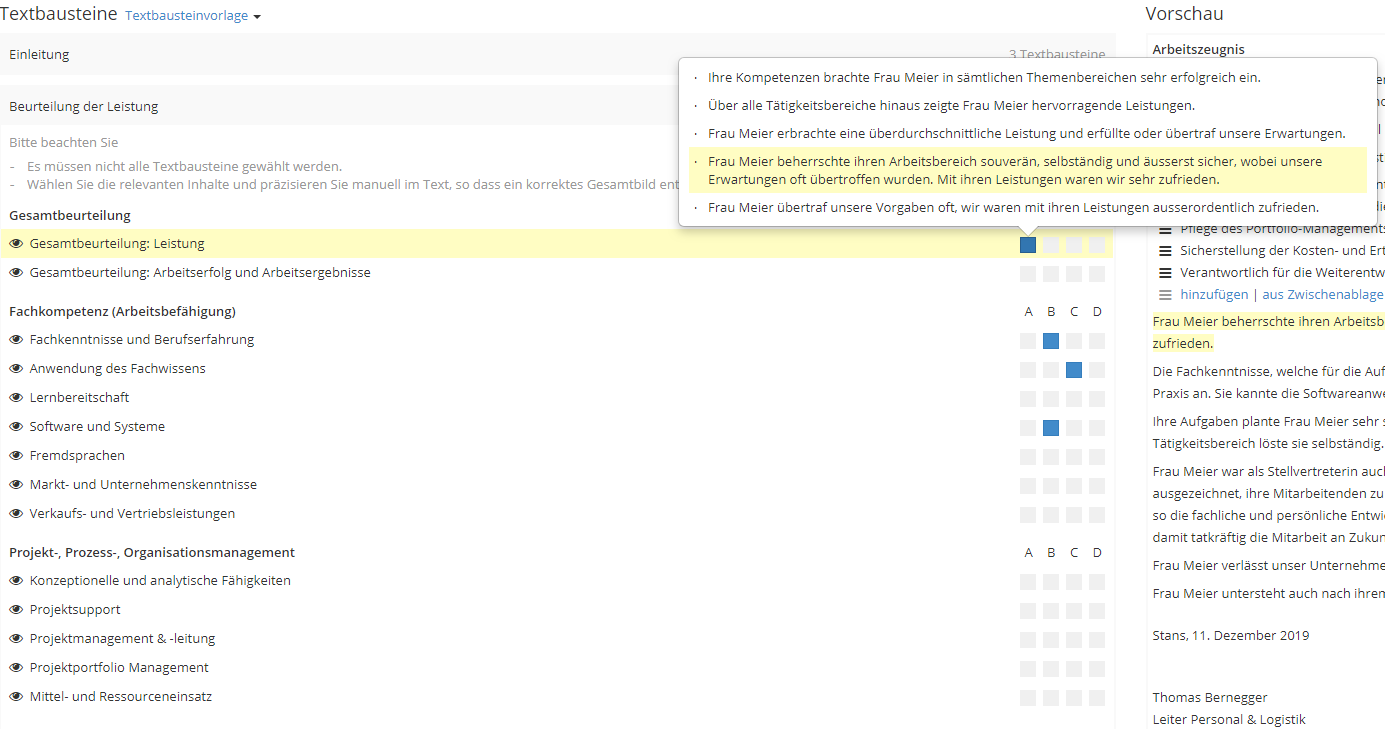
\includegraphics[scale=0.275]{zeugnismanager_narrow.png}
	\caption{Screenshot Zeugnismanager}
	\label{fig:screenshot_zeugnismanager}
\end{figure}
\noindent
\newline
Dabei sind die unten aufgeführten Sätze Beispiele für eine Bewertungskategorie mit der Bewertung A.
\begin{enumerate}
	\setlength\itemsep{0em}
	\item \textit{Herr Foo schaffte die Voraussetzungen für ein leistungsförderndes Arbeitsklima und unterstützte aktiv den konstruktiven Austausch im Team.}
	\item \textit{Herr Foo schaffte die Voraussetzungen für ein konstruktives und leistungsförderndes Arbeitsklima.}
	\item \textit{Herr Foo schaffte die nötigen Voraussetzungen für ein leistungsförderndes Arbeitsklima und eine konstruktive Zusammenarbeit.}
\end{enumerate}

Für tiefere Bewertungen stehen oft weniger Textbausteine zur Verfügung.
\begin{enumerate}
	\setlength\itemsep{0em}
	\item \textit{Die Zusammenarbeit im Team förderte Herr Foo nicht mit dem nötigen Engagement.}
\end{enumerate}
\noindent
Ein beispielhaftes Arbeitszeugnis, welches mit dem Zeugnismanager erstellt wurde, ist im Anhang zu finden
\fullref{ch:beispiel_arbeitszeugnis}. Die meisten Kunden des Auftraggebers editieren nach dem Erstellen des Zeugnisses
den Text, um das holprige Lesen zu verhindern. Die Unternehmen können die Textbausteine frei editieren, um bereits beim
Erstellen der Zeugnisse den Lesefluss zu fördern. Ein qualitativ hochwertiges Arbeitszeugnis, kann aufgrund des
Datenschutzes nicht angehängt werden. Jedoch soll anhand einiger Beispielsätze gezeigt werden, welche Qualität
angestrebt werden soll.
\begin{enumerate}
	\setlength\itemsep{0em}
	\item \textit{Bei der Ausübung seiner Aufgaben zeichnet er sich aus durch eine äusserst selbständige und effiziente Arbeitsweise, Beharrlichkeit sowie hohes Qualitäts- und Kostenbewusstsein.}
	\item \textit{Herr Foo ist Neuerungen gegenüber \textbf{offen, erkennt} Innovationsmöglichkeiten und bringt konkret umsetzbare Ideen ein.}
	\item \textit{Er pflegt eine offene Kommunikationskultur und informiert \textbf{zeit- und stufengerecht.}}
\end{enumerate}
\noindent
Dabei ist auf die Verschachtlung und Referenzen in den einzeln Sätzen zu achten. In den Textbausteinen des
Zeugnismanagers beschränkt sich die Verschachtlung auf Aufzählungen.

\section{Lösungsansatz}
\label{sec:Lösungsansatz}
Für die Lösung der Aufgabenstellung könnten verschiedene Ansätze verwendet werden, siehe
\fullref{sec:empfehlung_zeugnismanager}. Die Arbeitszeugnis des Zeugnismanagers zeugen bereits von guter Qualität. Sie
vermögen es jedoch nicht mit der Qualität von individuell geschriebener Zeugnisse mitzuhalten.
\newline
\newline
Da der Zeugnismanager wie erwähnt bereits ein auf dem Markt konkurrenzfähiges Produkt ist, käme die Umgestaltung des
Manager oder der Textbausteine einer Weiterentwicklung gleich. Dies ist nach Absprache mit dem Auftraggeber und des
Betreuer nicht das Ziel dieser Arbeit. Es soll daher ein neuer Ansatz gesucht werden, welcher ein Alleinstellungsmerkmal
für die Marktlösung des Auftraggebers sein kann. Weiter soll der Lösungsansatz im Bereich des maschinellen Lernen
angesiedelt sein, siehe \fullref{ch:aufgabenstellung}.
\newline
\newline
Für das Errechnen der Modelle ist ein grosser Datensatz nötig. Die Daten sollten dabei aus dem entsprechenden
Anwendungsgebiet stammen. Für die Umsetzung solcher Lösungen sind im Falle für Arbeitszeugnisse bedauerlicherweise nicht
genügend Daten vorhanden. Für die Arbeit soll daher ein Datensatz aufgebaut werden, welches das Problem abbildet. Anhand
des Datensatzes sollen Modelle für die Problemlösung evaluiert werden. Die Modelle sollen dabei den Style Transfer
vornehmen. Daher wurde entschieden einen Datensatz aufzubauen, welcher das Problem abbildet. Wie in
\fullref{sec:Problemdefinition} beschrieben geht es darum den Stil eines Satzes zu ändern. Es wird nun nach Daten
gesucht, die aus dem selben Themengebiete stammen und verschiedene Schreibstile aufweisen. Dabei werden die Stillabels $
holprig $ und $ flüssig $ durch Stillabels des verwendeten Datensatzes ersetzt. Der Datensatz sowie die neuen Stillabel
werden in \fullref{sec:verwendeter_datensatz} beschrieben.

\section{Evaluierung}
\label{sec:method_eval}
Die Evaluierung der Arbeit ist einer der wichtigsten Punkte des Projektes, denn dadurch soll festgestellt werden ob die
verfolgten Ansätze zum Lösen des Problemstellung vielversprechend sind und diese weiter verfolgt werden sollen.
\newline
\newline
Eine weiter Methode zur Überprüfung, ist die Messung der Verteilung des Datensatzes vor und nach dem Transfer. Damit
soll überprüft werden ob sich die Verteilung nach dem Transfer deutlich von der Vorherigen unterscheidet. Die neue
Verteilung sollte aufzeigen, dass die Sätze vor allem länger werden. Jedoch kann die Komplexität der
einzelnen Sätze nur schlecht statistisch gemessen werden und muss daher manuell gemacht werden.
\newline
\newline
Weiter sollen die Sätze manuell überprüft werden. Dabei werden diese vor und nach dem Transfer genauer betrachtet. So
kann abgeschätzt werden ob der Satz korrekt in die neue Domäne gebracht wurde. Ausserdem soll auf die Grammatik der
generierten Sätze geachtet werden um zu beurteilen ob diese korrekt erlernt wurde.

\section{Testing}
\label{sec:methode_test}
Um die Funktionsfähigkeit der Modelle sicherzustellen müssen diese automatisiert und nachvollziehbar getestet werden
können. Um diese Art von Testing zu gewährleisten, werden Unit Tests (\cite{unit_test}) verwendet. Diese können automatisiert ausgeführt
werden und testen immer den gleichen Ablauf mit vordefinierten Parametern. Unit Tests sollten immer nur einen Fall
testen, was in diesem Projekt auch so umgesetzt wurde.
\newline
\newline
Jedes verwendete Modell wird separat mit den gleichen Testfällen auf Richtigkeit überprüft. Die Modelle werden auf vier
solcher Testcases überprüft:
\begin{enumerate}
	\setlength\itemsep{0em}
	\item Testen ob die trainierbaren Variablen sich nach einem Trainingsschritt verändern
	\item Testen ob der Loss nach einem Trainingsschritt nicht Null ist
	\item Testen ob der Diskriminator separat von dem Generator trainiert werden kann
	\item Testen ob das Modell einen Output liefert
\end{enumerate}
\noindent
Durch diese vier Testfälle kann sichergestellt werden, dass das Modell trainiert werden kann und keinen Fehler in
der Architektur vorhanden sind und die einzelnen Schichten korrekt miteinander verbunden sind. Ausserdem kann durch
Testcase $3$ vergewissert werden, dass bei einem \gls{GAN} die beiden Komponenten separat voneinader trainiert werden
können. Jeder einzelne dieser Testfälle muss korrekt durchlaufen nach einer Änderung des Modells und am Schluss des
Projektes.

\section{Aufbau Projekt}
\label{sec:aufbau_projekt}
Das Projekt wurde in vier verschiedene Git Repositories unterteilt, um die einzelnen Schritte der Umsetzung sinnvoll zu
trennen. Diese werden im folgenden Abschnitt genauer beschrieben.

\subsection{wipro-doc}
\label{sub:wipro-doc}
In diesem Repository befindet sich die ganze Dokumentation des Projektes, sowie das Verzeichnis welches für die
Recherche der Arbeit gebraucht wird. Dieses Repository wird immer wieder bearbeitet und beinhaltet schlussendlich auch
die finale Dokumentation, welche abgegeben wird.
\newline
Link zum Git Repository: \hyperlink{https://gitlab.enterpriselab.ch/Pwn3rs/wipro-doc}{wipro-doc}
\newline
\dirtree{%
.1 wipro-doc.
.2 assets \ldots{} (assets for the project).
.2 documentation \ldots{} (latex file for final documentation).
.2 research \ldots{} (markdown file for research).
.2 study-doc \ldots{} (origin of study-doc).
}

\subsection{wipro-data}
\label{sub:wipro-data}
Wird verwendet, um die ganzen Daten, welche im Projekt genutzt werden, an einem zentralen Ort zu speichern. Darin sind
mehrere Datensätze vorhanden, welche im Repository aufbereitet und statistisch analysiert werden. Dieses Git Projekt ist
ein Git LFS Repository, da es sich um grosse Files handelt.
\newline
Link zum Git Repository: \hyperlink{https://gitlab.enterpriselab.ch/Pwn3rs/wipro-data}{wipro-data}
\newline
\dirtree{%
.1 wipro-data.
.2 utils \ldots{} (util classes for cleaning, processing the data).
.2 cleaned \ldots{} (cleaned data).
.2 crawled \ldots{} (crawled data).
.2 notebooks \ldots{} (jupyter notebooks for prepare, process and analyze data).
.2 processed \ldots{} (processed data).
.2 statistics \ldots{} (statistic data).
}

\subsection{wipro-source}
\label{sub:wipro-source}
Dieses Projekt beinhaltet die ganze Codebasis dieser Projektarbeit. Es ist dafür da, um verschiedene Modelle zu testen
und zu evaluieren. Darin befinden sich auch Datensätze von \textit{wipro-data}, um die entsprechenden Modelle damit zu
trainieren. In diesem Repository befindet sich ausserdem der Prototyp der Arbeit.
\newline
Link zum Git Repository: \hyperlink{https://gitlab.enterpriselab.ch/Pwn3rs/wipro-source}{wipro-source}
\newline
\dirtree{%
.1 wipro-source.
.2 data \ldots{} (data to train the models).
.2 dataloader \ldots{} (loads data for the models to process).
.2 network \ldots{} (architecture of the models).
.2 notebooks \ldots{} (jupyter notebooks to analyze models).
.2 save-model \ldots{} (saved models).
.2 test \ldots{} (unit tests for the networks).
.2 prototype.py \ldots{} (prototype of the project).
}

\subsection{wipro-logs}
\label{sub:wipro-logs}
In diesem Git Projekt befinden sich Log Files, Tensorboard Daten und Testsätze aller trainierten
Modelle. Dies wird zum Hyperparametertuning sowie zur Evaluierung gebraucht. In diesem Repository kann Tensorboard
gestartet werden und somit die entsprechenden Graphen eingesehen werden. Zu jedem trainierten Modell gibt es im
\textit{logs} Ordner ein entsprechende Verzeichnis mit den Daten.
\newline
Link zum Git Repository: \hyperlink{https://gitlab.enterpriselab.ch/Pwn3rs/wipro-logs}{wipro-logs}
\newline
\dirtree{%
.1 wipro-logs.
.2 log-archive \ldots{} (archive of the first models trained logs).
.2 logs \ldots{} (logs of the trained models).
.3 Classifier \ldots{} (logs of the classifiers).
.3 ControlGen \ldots{} (logs of the ControlGen models).
.3 CrossAlign \ldots{} (logs of the CrossAlign models).
.2 Tensorboard.ipynb \ldots{} (jupyter notebook to start tensorboard).
}
